%! TEX program = xelatex
\documentclass[a4paper]{article}
\usepackage{amsmath, amssymb, mathtools}
\usepackage{amsthm}
\usepackage{fontspec}
\usepackage{xunicode}
\usepackage{fancyhdr}
\usepackage[french]{babel}
\usepackage[a4paper,centering]{geometry}
\usepackage{algorithm, algorithmic}
\usepackage{listings}
\usepackage{color}
\usepackage{graphicx}
\usepackage{enumitem}
\usepackage[export]{adjustbox}
\usepackage{multicol}


\fancyhead[L, C, R]{}
\fancyfoot[L, R]{}
\fancyfoot[C]{\vspace{1mm}\thepage}
\renewcommand{\headrulewidth}{1pt}
\renewcommand{\footrulewidth}{1pt}
\pagestyle{fancy}

\definecolor{gray}{rgb}{0.94, 0.94, 0.94}
\definecolor{red}{rgb}{0.6, 0, 0}

\lstset{
    numbers=left,
    numberstyle=\tiny, 
    backgroundcolor=\color{gray},
    language=Python,
    keywordstyle=\color{red},
    breaklines=true,
    frame=leftline,
    tabsize=4,
}

\begin{document}

\thispagestyle{plain}

\begin{titlepage}
    \begin{center}

        \bigskip
        
\includegraphics[scale=0.5]{logo_su.jpg}~\\[4cm]

        {\LARGE Rapport du projet LU2IN013}\\[0.3cm]
        \rule{\linewidth}{0.5mm} \\[0.6cm]
        {\huge \textbf{Composition modulaire des polynômes à une variable}}\\[0.4cm]
        \rule{\linewidth}{0.5mm} \\[1cm]
        {\large Encadrant : M. Vincent NEIGER}\\[5cm]

        {\Large Serigne Fallou FALL, Marie BONBOIRE}
        
        \vfill
        Février 2023 - Juin 2023


    \end{center}
\end{titlepage}

\newpage

\tableofcontents

\newpage


\section{INTRODUCTION}
\subsection{Sujet}
\subsection{Objectifs}
\subsection{Choix d'implantation}


\section{NOTIONS ET NOTATIONS}


\subsection{Arithmétique modulaire}

\begin{itemize}[label=$\star$]
 \item Corps d'étude : ${\mathbb{Z}/p \mathbb{Z}}$
Notre étude porte principalement sur les opérations des polynomes dans l'anneau $Z/pZ$ , où p est un nombre premier, on travaille avec des polynômes à coefficients modulo p. Cela présente plusieurs avantages comme :
	\begin{itemize}

  		\item réduction des calculs à des opérations arithmétiques plus simples sur des entiers avec le modulo p.
  		\item simplification et limitations de la taille des coefficients pour obtenir des résultats plus facilement et permet d'exploiter des propriétés spécifiques de l'arithmétique modulaire.
  
	\end{itemize}
	
 \item Division euclidienne

\end{itemize}

- O tilde
- omega

\section{Multiplication}

Dans cette section, on étudie deux algorithmes qui calculent le produit de deux polynômes univariés.
Comprendre comment améliorer les performances d'un algorithme et les manipulations possibles sur les polynômes.


Soient deux polynômes $f$,g $\in \mathbb{Z}/p\mathbb{Z}[\mathrm{X}]$ de degré strictement inférieur à $n$ :
\[
f=f_0+f_1\mathrm{X}+...+f_{n-1}\mathrm{X}^{n-1}\text{ et g}=\mathrm{g}_0+\mathrm{g}_1\mathrm{X}+...+\mathrm{g}_{n-1}\mathrm{X}^{n-1}
\]

\subsection{Algorithme naif}

Ce premier algorithme consiste à simplement développer le produit des coefficients :
\[
f\cdot g=\sum_{i=0}^{2n-2} (\sum_{j+k=i}f_j\cdot g_k) x^i
\]

\subsubsection*{Complexité}
L'algorithme naïf est en $O(n^2)$

\begin{lstlisting}[title={multiplication naive}]
    def mult_naive(f, g) :
    ring = f.parent()

    #initialisation de la liste des coefficients
    res = [0]*(f.degree()+g.degree()+1) 
    
    for i in range(0, f.degree()+1):
        for j in range(0, g.degree()+1):
            res[i+j] += f[i]*g[j]

    return ring(res) 
\end{lstlisting}


\subsection{Algorithme de Karatsuba}

L'amélioration proposée par Karatsuba repose sur le fait de scinder les polynomes selon :
\[
f=f^{(0)}+f^{(1)}x^k\text{ et }g = g^{(0)}+g^{(1)}x^k
\]
avec $f^{(0)}, f^{(1)}, g^{(0)}, g^{(1)}$ de degré au plus $k-1$, $k=\lceil n/2 \rceil$. \\
Le produit s'écrit alors :
\[
  f\cdot g = (f^{(0)}\cdot g^{(0)})
  +\left((f^{(0)}+f^{(1)})\cdot (g^{(0)} + g^{(1)}) - f^{(0)}\cdot g^{(0)} - f^{(1)}\cdot g^{(1)}\right)x^k+
  (f^{(1)}\cdot g^{(1)})x^{2k} 
\]

Cette décomposition permet de gagner une multiplication par rapport à l'algorithme naïf. Notons que si $k=n$ on retombe sur l'algorithme naïf.

\begin{lstlisting}[title={Karatsuba}]
def karatsuba(f, g) :
    ring = f.parent()

    #cas de base
    if f.is_zero() : return f
    if g.is_zero() : return g
    
    #seuil à partir duquel la multiplication naïve est plus performante
    if (f.degree() <= 10 and g.degree() <= 10) : 
        return mult_naive(f, g)

    k = max(f.degree()/2, g.degree()/2).ceil()

    #extraction des sous polynômes
    f0 = ring(f.list()[:k]); f1 = ring(f.list()[k:])
    g0 = ring(g.list()[:k]); g1 = ring(g.list()[k:])

    #opérations de l'algorithme
    h1 = karatsuba(f0, g0)
    h2 = karatsuba(f1, g1)
    h5 = karatsuba(f0+f1, g0+g1)
    h7 = h5 - h1 - h2

    h = h1 + h7.shift(k) + h2.shift(2*k)

    return h
\end{lstlisting}

\subsubsection*{Complexité}
\begin{itemize}
    \item On calcule récursivement 3 multiplications de polynomes de degré au plus $k-1$
    \item 
\end{itemize}
Ainsi, l'algorithme de Karatsuba est en $O(n^{log_2(3)}) = O(n^{1,59})$

\subsection{Comparaisons}

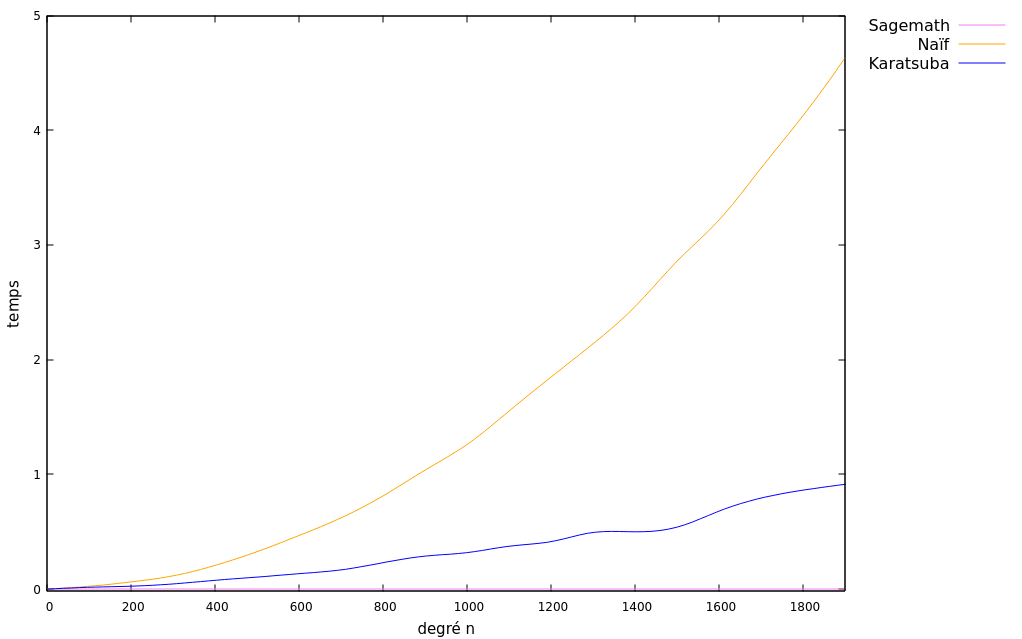
\includegraphics[scale=0.5, center]{multi.png}

\section{ALGORITHMES DE COMPOSITION MODULAIRE}

Dans cette autre section du rapport, on s'intéresse à l'étude et la comparaison de trois algorithmes de composition modulaire qui calculent g(a) mod f avec 
$f,g \in \mathbb{Z}/p\mathbb{Z}[\mathrm{X}]$ de degré $n$ et a de degré $< n$.



\subsection{Algorithme naïf}

L'algorithme naïf de composition modulaire consiste à directement évaluer g en a et à retourner le résultat en le réduisant par f :
\[
g(a)\text{ mod }f = \left(\sum_{k=0}^n g_k \cdot a^k\right) \text{ mod }f    
\]

\begin{lstlisting}[title={naive}]
def eval_naive(g, a, f) :
	ring = g.parent()

	res = ring(g[0])
	ai = a
	
    for i in range(1, g.degree()+1) :
		res = res + g[i]*ai
		ai = (a*ai)

	return res % f
\end{lstlisting}

\subsubsection*{Complexité}
\begin{itemize}
    \item Pour $i \in \{0,...,n\}$, le degré des $a_i$ est au plus égal à $k(n-1)$ donc, le produit $a_i=a_{i-1}\cdot a$ est en $\tilde{O}(kn)$
    \item On effectue $n$ tours de boucles donc $n$ multiplications
\end{itemize}
Ainsi, la complexité de l'algotihme naïf est :
\[
\sum_{k=1}^{n}kn=n \cdot \dfrac{n(n+1)}{2} \Longrightarrow \tilde{O}(n^3)
\]

\subsection{Algorithme d'Horner}

\[
g(a)\text{ mod }f = ((...((((g_{n-1}\cdot a)\text{ mod }f\ +\ g_{n-2})\cdot a)\text{ mod }f\ +\ g_{n-3})...)\cdot a)\text{ mod }f\ +\ g_0
\]

\begin{lstlisting}[title={Horner}]
    def horner(g, a, f) :
        res = g[g.degree()]
        for i in range(g.degree()-1, -1, -1) :
            res = (res*a)%f + g[i]
        return res%f
    \end{lstlisting}

\subsubsection*{Complexité}
\begin{itemize}
    \item Pour $i \in \{0,...,n\}$, le degré de $a_i$ mod $f$ est au plus égal à $n$ donc, le produit $a_i=a_{i-1}\cdot a$ est en $\tilde{O}(n)$
    \item On effectue $n$ tours de boucles donc $n$ multiplications
\end{itemize}
Ainsi, la complexité de l'algorithme d'Horner est :
\[
\sum_{i=1}^n n=n\cdot \sum_{i=1}^n 1 = n\cdot n\Longrightarrow \tilde{O}(n^2)
\]

\subsection{Algorithme de Brent et Kung}

L'avancée de Brent et Kung a été de considérer le produit bien connu de deux matrices à coefficients constants $\omega$.


En choissant $\delta = \sqrt(n)$, il est possible de réécrire $g$ sous la forme de :
\begin{align*}
    g(y) &= g_0 + g_1y + ... + g_{\delta-1}y^{\delta-1} \\
        &+ y^\delta(g_\delta + g_{\delta+1}y + ... + g_{2\delta-1}y^{\delta-1}) \\
                                      &+ y^{2\delta}(g_{2\delta} + g_{2\delta+1}y + ... + g_{3\delta-1}y^{\delta-1}) \\
                                      &+ ... \\
                                      &+ y^{\delta(\delta-1)}(g_{\delta(\delta-1)} + g_{\delta(\delta-1)+1}y + ... + g_{\delta^2-1}y^{\delta-1}) 
\end{align*}

Il est alors possible de transformer cette expression en produit de matrices dont une est à coefficients constants:
\[
g(y) = 
\begin{pmatrix}
    1 & y^\delta & ... & (y^\delta)^{\delta-1}  \\  
\end{pmatrix}
\begin{pmatrix}
    g_0 & g_1 & ... & g_{\delta-1} \\
    g_{\delta} & g_{\delta+1} & ... & g_{2\delta-1} \\
    \vdots & ... & \vdots \\
    g_{\delta(\delta-1)} & g_{\delta(\delta-1)+1} & ... & g_{\delta^2-1}
\end{pmatrix}
\begin{pmatrix}
    1 \\
    y \\
    \vdots \\
    y^{\delta-1}
\end{pmatrix}
\]

De même, on transforme le vecteur des $\delta$ puissances de $a$ mod $f$, en un produit d'une matrice à coefficients constants par un vecteur de l'inconnue, soit $x$ :
\[
    \begin{pmatrix}
        1 \\
        a \text{ mod }f\\
        \vdots \\
        a^{\delta-1} \text{ mod }f
    \end{pmatrix}
    =
    \begin{pmatrix}
        1 & 0 & ... & 0 \\
        a_{1,0} & a_{1,1} & ... & a_{1,n-1} \\
        \vdots & \vdots & ... & \vdots \\
        a_{\delta-1,0} & a_{\delta-1,1} & ... & a_{\delta-1,n-1}
    \end{pmatrix}
    \begin{pmatrix}
        1 \\
        x \\
        \vdots \\
        x^{n-1}
    \end{pmatrix}
\]

On obtient ainsi la formule suivante :
\[
g(a)\text{ mod }f =
\begin{pmatrix}
    1 & y^\delta & ... & (y^\delta)^{\delta-1}  \\  
\end{pmatrix}
\begin{pmatrix}
    g_0 & ... & g_{\delta-1} \\
    g_{\delta} & ... & g_{2\delta-1} \\
    \vdots & ... & \vdots \\
    g_{\delta(\delta-1)} & ... & g_{\delta^2-1}
\end{pmatrix}
\begin{pmatrix}
    1 &  ... & 0 \\
    a_{1,0} & ... & a_{1,n-1} \\
    \vdots &  ... & \vdots \\
    a_{\delta-1,0} & ... & a_{\delta-1,n-1}
\end{pmatrix}
\begin{pmatrix}
    1 \\
    x \\
    \vdots \\
    x^{\delta-1}
\end{pmatrix}
\]


\begin{lstlisting}[title={brent and kung}]
def brentkung(g, a, f) :

	ring = a.parent()
	d = g.degree()+1; n = f.degree()
	if a.degree() >= n:
		raise ValueError("Erreur: a de degré trop élevé")

	r = RR(d.sqrt()).ceil()
	s = RR(d/r).ceil()

    #calcul des puissances de a
	ac = [ring(0)]*(r+1)
	ac[0] = ring(1)
	for i in range(1, r+1) :
		ac[i] = (a*ac[i-1]) % f

    #calcul du produit matriciel
	ma = matrix(r, n, [(ac[i])[j] for i in range(r) for j in range(n)])
	mg = matrix(s, r, [g[i*r+j] for i in range(s) for j in range(r)])
	mb = mg*ma

    #liste coefficients -> polynôme
	b = [ring(0)]*s
	for i in range(s) :
		b[i] = ring(mb[i].list())

	res = b[0]
	ar = ac[r]

	res = horner(b, ar, f)
	return res
\end{lstlisting}

\subsubsection*{Complexité}
\begin{itemize}
    \item Pour $i \in \{0,...,n\}$, le degré des $a_i$ est au plus égal à $k(n-1)$ donc, le produit $a_i=a_{i-1}\cdot a$ est en $\tilde{O}(kn)$
    \item On effectue $n$ tours de boucles donc $n$ multiplications
\end{itemize}

\newpage

\subsection{Comparaisons}
\begin{multicols}{2}
    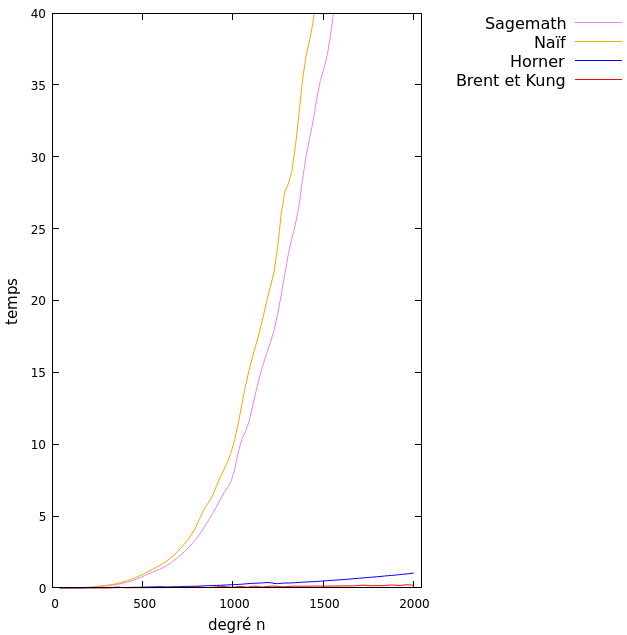
\includegraphics[scale=0.4, center]{comp.png}
    \columnbreak

    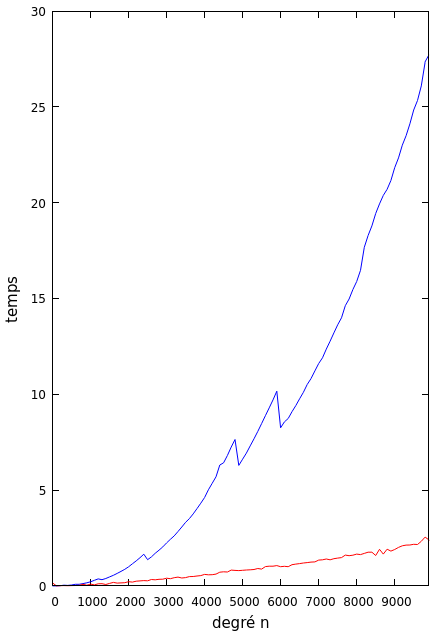
\includegraphics[scale=0.4, center]{comp_2.png}
\end{multicols}

\section{ALGORITHME DE NUSKEN ET ZIEGLER}

L'algorithme de Nüsken et Ziegler est une généralisation de celui de Brent et Kung aux polynômes à deux variables. 
Son principe est donc similaire, en différant au niveau de la matrice des coefficients de $g$ qui ici, contient des polynomes en $x$.
On y retrouve toutefois les mêmes étapes de calcul.

\[
g(x,y) = \sum_{i,j<\delta}g_{i+\delta j}(x)y^{i+\delta j} = \sum_{j<\delta} \left( \sum_{i<\delta} g_{i+\delta j}(x)y^i \right) y^{\delta j}     
\]
\[
g(x, a)\text{ mod }f =
\begin{pmatrix}
    1 & y^\delta & ... & (y^\delta)^{\delta-1}  \\  
\end{pmatrix}
\begin{pmatrix}
    g_0(x) & ... & g_{\delta-1}(x) \\
    g_{\delta}(x) & ... & g_{2\delta-1}(x) \\
    \vdots & ... & \vdots \\
    g_{\delta(\delta-1)}(x) & ... & g_{\delta^2-1}(x)
\end{pmatrix}
\begin{pmatrix}
    1 &  ... & 0 \\
    a_{1,0} & ... & a_{1,n-1} \\
    \vdots &  ... & \vdots \\
    a_{\delta-1,0} & ... & a_{\delta-1,n-1}
\end{pmatrix}
\begin{pmatrix}
    1 \\
    x \\
    \vdots \\
    x^{\delta-1}
\end{pmatrix}
\]

\begin{lstlisting}[title={nusken et ziegler}]
def nusken(g, a, f) :
    ring = a.parent()
    d = RR(sqrt(g.degree()+1)).ceil()

    #réécriture
    ringY = g.parent().univariate_ring(y)
    lg = ringY(g)

    #calcul du produit matriciel
    mg = matrix(d, d, [lg[i+d*j](X) for j in range(d) for i in range(d) ])

    ac = [ring(0)]*d
    ac[0] = ring(1)
    for i in range(1, d) :
        ac[i] = (a*ac[i-1]) % f

    ma = vector(ac)
    
    mr = mg*ma

    r = [ring(0)]*d
    for j in range(d) :
        r[j] = ring(mr[j].list()) %f
    
    #calcul des autres puissances de a
    aj = [ring(0)]*d
    for j in range(d) :
        aj[j] = a**(d*j) %f

    #calcul du resultat
    res = ring(0)
    for j in range(d) :
        res += r[j]*aj[j] %f

    return res

\end{lstlisting}

\newpage
\section{BIBLIOGRAPHIE}

\nocite{*}

\bibliographystyle{plain}
\bibliography{biblio}


%\begin{thebibliography}{10}
%    \bibitem{aecf} Alin Bostan, Frédéric Chyzak, Marc Giusti, Romain Lebreton, Grégoire Lecerf, Bruno Salvy, Eric Schost,
%    \emph{Algorithmes efficaces en calcul formel}, 2017
%
%\end{thebibliography}


\end{document}


